\section{Zugriff auf den Schlüsselbund durch Apps}

Wie bereits erläutert, ist der Schlüsselbund durch eine verschlüsselte SQLite-Datenbank realisiert, die im Dateisystem hinterlegt ist. Eine App kann den Schlüsselbund verwenden um Passwörter, Kreditkarteninformationen, Zertifikate, Identitäten oder auch kurze Notizen verschlüsselt zu hinterlegen \cite{apple2020keychain_services}.
Diesen Daten können Attribute zugeordnet werden, welche nicht verschlüsselt sind, sodass die Daten auch nach der Verschlüsselung im Schlüsselbund gefunden werden können \cite{apple2020keychain_items}. 

\begin{figure}[h]
	\centering
  		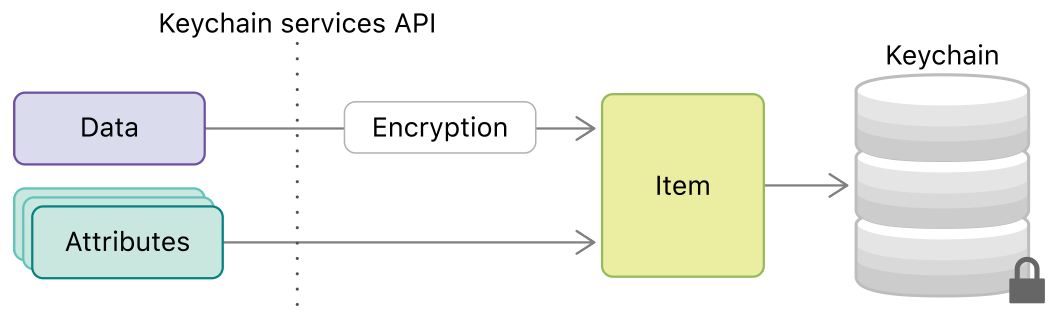
\includegraphics[width=1\textwidth]{../images/keychain-api-example}
		\caption{Hinzufügen eines Eintrags zu dem Schlüsselbund durch App \cite{apple2020keychain_items}}
		\label{fig:add-entry-to-keychain}
\end{figure}

Der Zugriff durch eine App auf den Schlüsselbund geschieht durch den \textit{securityd}-Daemon (Abb. \ref{fig:add-entry-to-keychain}). Dieser bietet eine API zum Speichern beziehungsweise Verschlüsseln und Auslesen von Schlüsselbundeinträgen. Zudem  entscheidet der Deamon auf Basis der Berechtigung \textit{keychain-access-groups}, welche App auf welchen Eintrag im Schlüsselbund zugreifen darf. Durch die Klassifizierung der Apps in Gruppen, können Informationen innerhalb dieser Gruppen ausgetauscht werden \cite{apple2020keychain_item_groups}. Somit muss ein*e Nutzer*in sich nur in einer von zwei oder mehr zusammenhängenden Apps authentifzieren und ist unmittelbar auch in den anderen der Gruppe zugehörigen Apps angemeldet. Als Voraussetzung gilt auch hier, dass die Apps von dem gleichen Entwickler*innenteam veröffentlicht wurden. \\
Apps die neben dem Schlüsselbund auch weitere Daten austauschen möchten, sind einer \textit{application-group} zugehörig.  Somit können gemeinsame Container verwendet oder durch eine Interprozesskommunikation Informationen ausgetauscht werden \cite{apple2020keychain_application_groups}. 

